\documentclass[../main.tex]{subfiles}
\graphicspath{{\subfix{../images/}}}
\begin{document}

\subsection*{Answers - King rule for integration (page \pageref{Kings rule})}
\label{Kings rule answers}
\begin{enumerate}[itemsep=0.7cm]
    \setstretch{1.5}
    \item 
    $\int_0^{\frac{\pi}{2}}\frac{\sin^n{(x)}}{\sin^n{(x)}+\cos^n{(x)}}\,dx$

    $\frac{1}{2}\int_0^{\frac{\pi}{2}}\frac{\sin^n{(x)}}{\sin^n{(x)}+\cos^n{(x)}}+\frac{\sin^n{(\frac{\pi}{2}-x)}}{\sin^n{(\frac{\pi}{2}-x)}+\cos^n{(\frac{\pi}{2}-x)}}\,dx$

    $\frac{1}{2}\int_0^{\frac{\pi}{2}}\frac{\sin^n{(x)}}{\sin^n{(x)}+\cos^n{(x)}}+\frac{\cos^n{(x)}}{\cos^n{(x)}+\sin^n{(x)}}\,dx$

    $\frac{1}{2}\int_0^{\frac{\pi}{2}}\frac{\sin^n{(x)}+\cos^n{(x)}}{\sin^n{(x)}+\cos^n{(x)}}\,dx$

    $\frac{1}{2}\int_0^{\frac{\pi}{2}}1\,dx$

    $\frac{1}{2}\times \frac{\pi}{2}=\frac{\pi}{4}$

    \item 
    $\int_0^{\frac{\pi}{2}}\frac{1}{1+(\tan{x})^{\pi}}\,dx$

    $\frac{1}{2}\int_0^{\frac{\pi}{2}}\frac{1}{1+(\tan{x})^{\pi}}+\frac{1}{1+\bigl(\tan{(\frac{\pi}{2}-x)}\bigr)^{\pi}}\,dx$

    Cotangent is the complement of tangent, therefore $\tan{(\frac{\pi}{2}-x)}=\cot{x}=\frac{1}{\tan{x}}$

    $\frac{1}{2}\int_0^{\frac{\pi}{2}}\frac{1}{1+(\tan{x})^{\pi}}+\frac{1}{1+\bigl(\frac{1}{\tan{x}}\bigr)^{\pi}}\,dx$

    Simplifying:

    $\frac{1}{2}\int_0^{\frac{\pi}{2}}\frac{1}{1+(\tan{x})^{\pi}}+\frac{1}{1+\bigl(\frac{1}{\tan{x}}\bigr)^{\pi}}\times \frac{(\tan{x})^{\pi}}{(\tan{x})^{\pi}}\,dx=\frac{1}{2}\int_0^{\frac{\pi}{2}} \frac{1}{1+(\tan{x})^{\pi}}+\frac{(\tan{x})^{\pi}}{(\tan{x})^{\pi}+1}\,dx$

    $\frac{1}{2}\int_0^{\frac{\pi}{2}} \frac{1+1+(\tan{x})^{\pi}}{1+(\tan{x})^{\pi}}$

    $\frac{1}{2}\int_0^{\frac{\pi}{2}} 1\,dx$

    $\frac{1}{2}\times \frac{\pi}{2}=\frac{\pi}{4}$

    \item 
    $\int_0^1 \frac{\ln{(x+1)}}{x^2+1}\,dx$
    
    Using a trig substitution first:

    \begin{figure}[h]
        \centering
        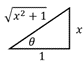
\includegraphics{images/trigsuba8.png}
    \end{figure}

    $\tan{\theta}=x$

    $\sec^2{\theta}\,d\theta=dx$

    Upper bound changes to $\frac{\pi}{4}$.

    $\int_0^{\frac{\pi}{4}} \frac{\ln{(\tan{\theta}+1)}}{\tan^2{\theta}+1}\sec^2{\theta}\,d\theta=\int_0^{\frac{\pi}{4}} \frac{\ln{(\tan{\theta}+1)}}{\sec^2{\theta}}\sec^2{\theta}\,d\theta=\int_0^{\frac{\pi}{4}} \ln{(\tan{\theta}+1)}\,d\theta$

    Now we apply the King rule:

    $\frac{1}{2}\int_0^{\frac{\pi}{4}} \ln{(\tan{\theta}+1)}+\ln\bigl[(\tan{(\frac{\pi}{4}-\theta)}+1)\bigr]\,d\theta$

    Use the tangent compound angle rule:

    $\tan{(\frac{\pi}{4}-\theta)}=\frac{\tan{\frac{\pi}{4}}-\tan{\theta}}{1+\tan{\frac{\pi}{4}}\tan{\theta}}=\frac{1-\tan{\theta}}{\tan{1+\theta}}$

    So the definite integral becomes:

    $\frac{1}{2}\int_0^{\frac{\pi}{4}} \ln{(\tan{\theta}+1)}+\ln\Bigl[\frac{1-\tan{\theta}}{1+\tan{\theta}}+1\Bigr]\,d\theta$

    $\frac{1}{2}\int_0^{\frac{\pi}{4}} \ln{(\tan{\theta}+1)}+\ln\Bigl[\frac{1-\tan{\theta}}{1+\tan{\theta}}+\frac{1+\tan{\theta}}{1+\tan{\theta}}\Bigr]\,d\theta$

    $\frac{1}{2}\int_0^{\frac{\pi}{4}} \ln{(\tan{\theta}+1)}+\ln\Bigl[\frac{2}{1+\tan{\theta}}\Bigr]\,d\theta$

    $\frac{1}{2}\int_0^{\frac{\pi}{4}} \ln{(\tan{\theta}+1)}+\ln{2}-\ln{(1+\tan{\theta})}\,d\theta$

    $\frac{1}{2}\int_0^{\frac{\pi}{4}} \ln{2}\,d\theta$

    $\frac{\ln{2}}{2}\int_0^{\frac{\pi}{4}} 1\,d\theta$

    $=\frac{\ln{2}}{2} \times \frac{\pi}{4}=\frac{\pi}{8}\ln{2}$

    \item 
    $\int_0^{\pi} \frac{x\sin{x}}{1+\sin{x}}\,dx$

    $\frac{1}{2}\int_0^{\pi} \frac{x\sin{x}}{1+\sin{x}}+\frac{(\pi-x)\sin{(\pi-x)}}{1+\sin{(\pi-x)}}\,dx$

    To keep the denominators the same and to eliminate the $x\sin{x}$, note that $sin{(\pi-x)}=\sin{x}$.

    $\frac{1}{2}\int_0^{\pi} \frac{x\sin{x}}{1+\sin{x}}+\frac{(\pi-x)\sin{x}}{1+\sin{x}}\,dx$

    $\frac{1}{2}\int_0^{\pi} \frac{x\sin{x}+\pi\sin{x}-x\sin{x}}{1+\sin{x}}\,dx=\frac{1}{2}\int_0^{\pi} \frac{\pi\sin{x}}{1+\sin{x}}\,dx$

    $\frac{\pi}{2}\int_0^{\pi} \frac{\sin{x}}{1+\sin{x}}\,dx$

    $\frac{\pi}{2}\int_0^{\pi} \frac{\sin{x}}{1+\sin{x}}\times \frac{1-\sin{x}}{1-\sin{x}}\,dx=\frac{\pi}{2}\int_0^{\pi} \frac{\sin{x}-\sin^2{x}}{1-\sin^2{x}}\,dx$

    Simplifying further:
    $\frac{\pi}{2}\int_0^{\pi} \frac{\sin{x}-\sin^2{x}}{\cos^2{x}}\,dx=\frac{\pi}{2}\int_0^{\pi} \frac{\sin{x}}{\cos^2{x}}-\frac{\sin^2{x}}{\cos^2{x}}\,dx$

    $\frac{\pi}{2}\int_0^{\pi} \frac{\sin{x}}{\cos^2{x}}-\tan^2{x}\,dx=\frac{\pi}{2}\int_0^{\pi} \frac{\sin{x}}{\cos^2{x}}\,dx-\frac{\pi}{2}\int_0^{\pi}\tan^2{x}\,dx$

    $\frac{\pi}{2}\int_0^{\pi} \frac{\sin{x}}{\cos^2{x}}\,dx-\frac{\pi}{2}\int_0^{\pi}\sec^2{x}-1\,dx$

    Separate into two integrals:

    $I_1=\frac{\pi}{2}\int_0^{\pi} \frac{\sin{x}}{\cos^2{x}}\,dx$

    $I_2=\frac{\pi}{2}\int_0^{\pi}\sec^2{x}-1\,dx$

    For $I_1$, use a substitution of $u=\cos{x}$:

    $du=-\sin{x}\,dx \rightarrow -du=\sin{x}\,dx$

    Bounds change to 1 and -1.

    $I_1=-\frac{\pi}{2}\int_1^{-1}u^{-2}\,du=\frac{\pi}{2}\int_{-1}^1 u^{-2}\,du$

    $I_1=\frac{\pi}{2}\Bigl[-\frac{1}{u}\Bigr]_{-1}^1=-\pi$

    $I_2=\frac{\pi}{2}\int_0^{\pi}\sec^2{x}-1\,dx=\frac{\pi}{2}\Bigl[\tan{x}-x\Bigr]_0^{\pi}=-\frac{\pi^2}{2}$

    $I=I_1 - I_2 = -\pi - -\frac{\pi^2}{2}=\frac{\pi^2}{2}-\pi$

\end{enumerate}


\pagebreak


\end{document}